\section{问题三模型的建立与求解}

\subsection{模型建立}

问题三将电氢氨装置的运行方式从离散开关改为功率连续可调（下限为额定功率的10\%）。各时段的制氢氨功率$p(t)$可在$[0.1P_{\mathrm{max}}, P_{\mathrm{max}}]$区间内连续调节，也可完全停机（$p(t)=0$）。这是一个连续线性规划问题。

定义连续变量$p(t)$为时段$t$的制氢氨功率：
\begin{equation}
p(t) \in \{0\} \cup [0.1P_{\mathrm{max}},\; P_{\mathrm{max}}], \quad t = 0,1,\ldots,23 \label{eq:q3_var}
\end{equation}
其中$P_{\mathrm{max}} = 41.5$ MW。

目标为最小化日净电费与运维成本之和：
\begin{equation}
\min \; F = \sum_{t=0}^{23} \bigl[ P_{\mathrm{b}}(t)C_{\mathrm{b}}(t) - P_{\mathrm{s}}(t)C_{\mathrm{s}} + C_{\mathrm{OM}}(t) \bigr] \label{eq:q3_obj}
\end{equation}
运维成本$C_{\mathrm{OM}}(t) = p(t) \times 126$元。

约束条件包括功率平衡、功率上下限和日产量约束：
\begin{align}
&P_{\mathrm{w}}(t) + P_{\mathrm{pv}}(t) + P_{\mathrm{b}}(t) = P_{\mathrm{L}}(t) + p(t) + P_{\mathrm{s}}(t) \quad \forall t \label{eq:q3_bal} \\
&p(t) \in \{0\} \cup [0.1P_{\mathrm{max}},\; P_{\mathrm{max}}] \quad \forall t \label{eq:q3_plim} \\
&\sum_{t=0}^{23} p(t) \cdot \eta = Q_{\mathrm{NH_3}}, \quad \eta = \frac{3.0}{41.5} = 0.0723 \; [\text{t/MWh}] \label{eq:q3_q}
\end{align}

整理为标准形式：
\begin{align}
\min \; & \sum_{t=0}^{23} \Bigl[ C_{\mathrm{b}}(t)\max\{P_{\mathrm{L}}(t) + p(t) - P_{\mathrm{w}}(t) - P_{\mathrm{pv}}(t),\; 0\} \notag \\
&\qquad - C_{\mathrm{s}}\max\{P_{\mathrm{w}}(t) + P_{\mathrm{pv}}(t) - P_{\mathrm{L}}(t) - p(t),\; 0\} + 126p(t) \Bigr] \label{eq:q3_model} \\
\text{s.t.} \quad & \sum_{t=0}^{23} p(t) \cdot \eta = Q_{\mathrm{NH_3}},\; p(t) \in \{0\} \cup [0.1P_{\mathrm{max}},\; P_{\mathrm{max}}],\; \forall t \notag
\end{align}

\subsection{模型求解}

\textbf{步骤一：计算各时段可再生盈余。}对每个时段$t$，计算风光出力扣除常规负荷后的剩余功率：
\begin{equation*}
\Delta P(t) = \max\{0,\; P_{\mathrm{w}}(t) + P_{\mathrm{pv}}(t) - P_{\mathrm{L}}(t)\}
\end{equation*}
这个盈余是可免费利用的可再生电力（若不利用只能以0.3779元/kWh的价格上网出售）。

\textbf{步骤二：优先利用盈余。}将盈余最大的时段按从大到小排序，逐时段分配制氢功率$p(t)$。对于每个时段，尽量利用盈余，但不超过设备最大功率41.5 MW且不低于最小功率4.15 MW：
\begin{equation*}
p(t) = \min\{\text{剩余需求},\; \Delta P(t),\; 41.5\}
\end{equation*}
若$\Delta P(t) < 4.15$ MW，则不在此时段分配功率（无法满足下限要求）。

\textbf{步骤三：不足部分按边际成本分配。}如果步骤二分配后仍有剩余产量需求，计算剩余时段开机的边际成本：
\begin{equation*}
\text{边际成本} = 
\begin{cases}
-377.9 + 126 = -251.9\ \text{元/MWh}, & \text{该时段可再生有盈余}\\
C_{\mathrm{b}}(t) + 126\ \text{元/MWh}, & \text{该时段需购电}
\end{cases}
\end{equation*}
其中$-377.9$是放弃售电的机会成本，$+126$是运维成本。按边际成本从小到大排序，逐时段分配功率。

以36吨/日目标为例，先分配盈余时段：
\begin{itemize}
    \item $t=12$，$\Delta P=57.3$ MW，可取满41.5 MW
    \item $t=11$，$\Delta P=50.1$ MW，可取满41.5 MW
    \item 依次分配盈余时段后，仍有少量剩余需求
\end{itemize}
然后将剩余需求量按边际成本最小的原则分配到$t=0-6$谷电价时段（购电价342.4元/MWh$+126=468.4$元/MWh）。

\textbf{步骤四：微调余量。}若最后剩余不足4.15 MW的功率需求，追加到已有运行时段上（在其现有功率基础上增加少量出力，确保总功率不超过41.5 MW），保证产量精确达标。

为了直观展示连续调节与离散调节在调度策略上的本质差异，以72吨/日满产为例，分别运行两种优化算法得到各时段的制氢氨功率安排、购电功率和售电功率，绘制对比图如\cref{fig:q3_schedule}所示。其中离散调节的功率曲线呈阶梯状（要么满发41.5 MW，要么停机0 MW），连续调节的功率曲线可连续变化。

\begin{figure}[H]
\centering
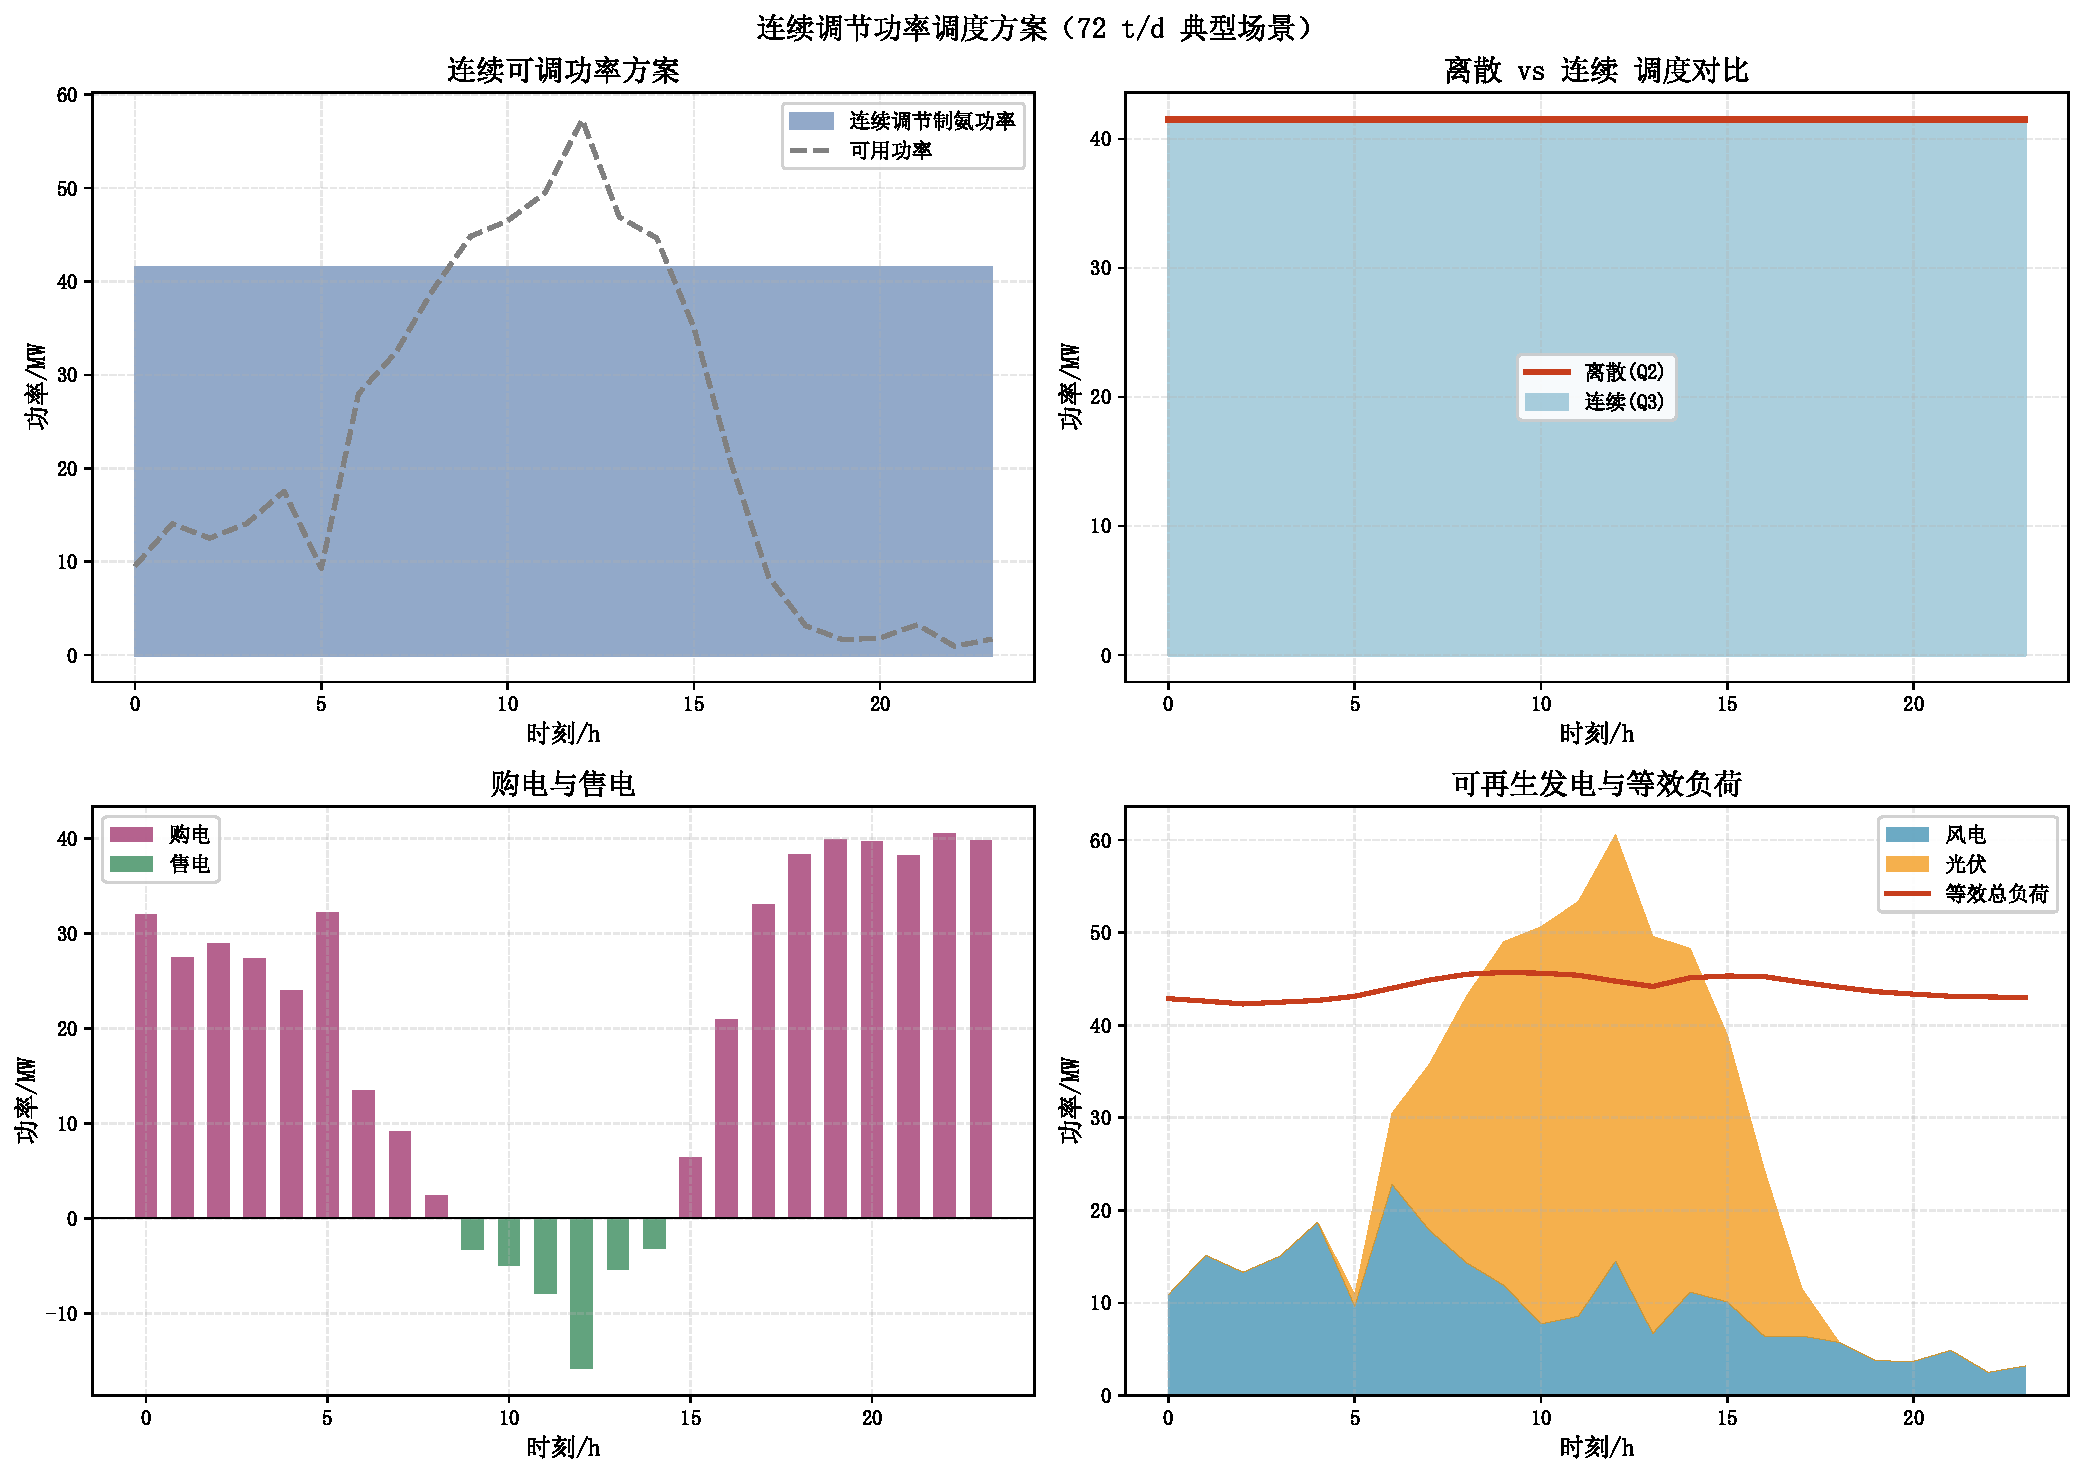
\includegraphics[width=\textwidth]{../figures/q3/fig9_q3_power_schedule.pdf}
\caption{连续调节功率调度方案（72 t/d典型场景）}
\label{fig:q3_schedule}
\end{figure}

\cref{fig:q3_schedule}对比了同一场景下离散和连续调节的差异。连续调节的制氨功率平滑跟随可再生出力，避免了购售电极端波动。

各产量下Q2与Q3的关键指标对比见\cref{tab:q3_comparison}。

\begin{table}[H]
\centering
\caption{Q2与Q3关键指标对比（典型场景）}
\label{tab:q3_comparison}
\begin{tabular*}{\textwidth}{@{\extracolsep{\fill}}ccccccc}
\toprule[1.5pt]
产量 & \multicolumn{2}{c}{吨氨成本(元/吨)} & \multicolumn{2}{c}{自用比例} & \multicolumn{2}{c}{上网比例} \\
(t/d) & Q2 & Q3 & Q2 & Q3 & Q2 & Q3 \\
\midrule[1pt]
72 & 6219 & 6219 & 86.5\% & 86.5\% & 6.7\% & 6.7\% \\
63 & 5328 & 5858 & 84.3\% & 84.6\% & 7.8\% & 7.7\% \\
54 & 4591 & 4758 & 80.2\% & 82.4\% & 9.9\% & 8.8\% \\
45 & 3945 & 4005 & 51.0\% & 82.4\% & 24.5\% & 8.8\% \\
36 & 3192 & 3406 & 10.5\% & 82.4\% & 44.7\% & 8.8\% \\
\bottomrule[1.5pt]
\end{tabular*}
\end{table}

\cref{tab:q3_comparison}显示连续调节在各产量下自用比例稳定在82\%以上，上网比例控制在9\%以内，显著优于离散调节。

以上对比仅基于典型日场景，不足以全面反映连续调节的优势。为进一步验证连续调节在多种天气条件下的表现，将6种风电场景与4种光伏场景两两组合得到24种风光场景，分别在离散和连续两种调节方式下进行优化。对每种场景的每个产量水平，计算其吨氨成本和绿电指标，与离散调节的结果进行逐场景对比。将各产量下24场景的成本均值和达标情况汇总，绘制Q2与Q3的成本对比图和达标统计对比图如\cref{fig:q10_comparison}和\cref{fig:q12_compliance}所示。

\begin{figure}[H]
\centering
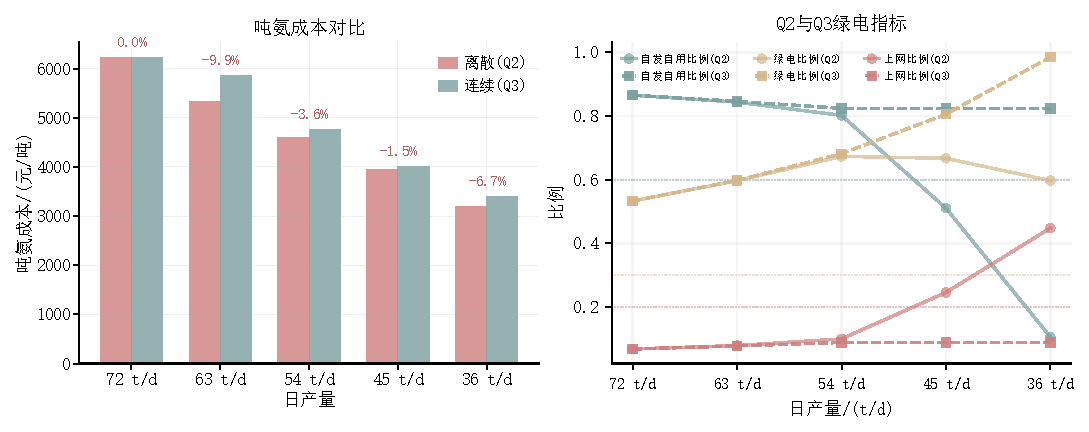
\includegraphics[width=\textwidth]{../figures/q3/fig10_q2_vs_q3.pdf}
\caption{Q2 vs Q3吨氨成本与绿电指标对比}
\label{fig:q10_comparison}
\end{figure}

\begin{figure}[H]
\centering
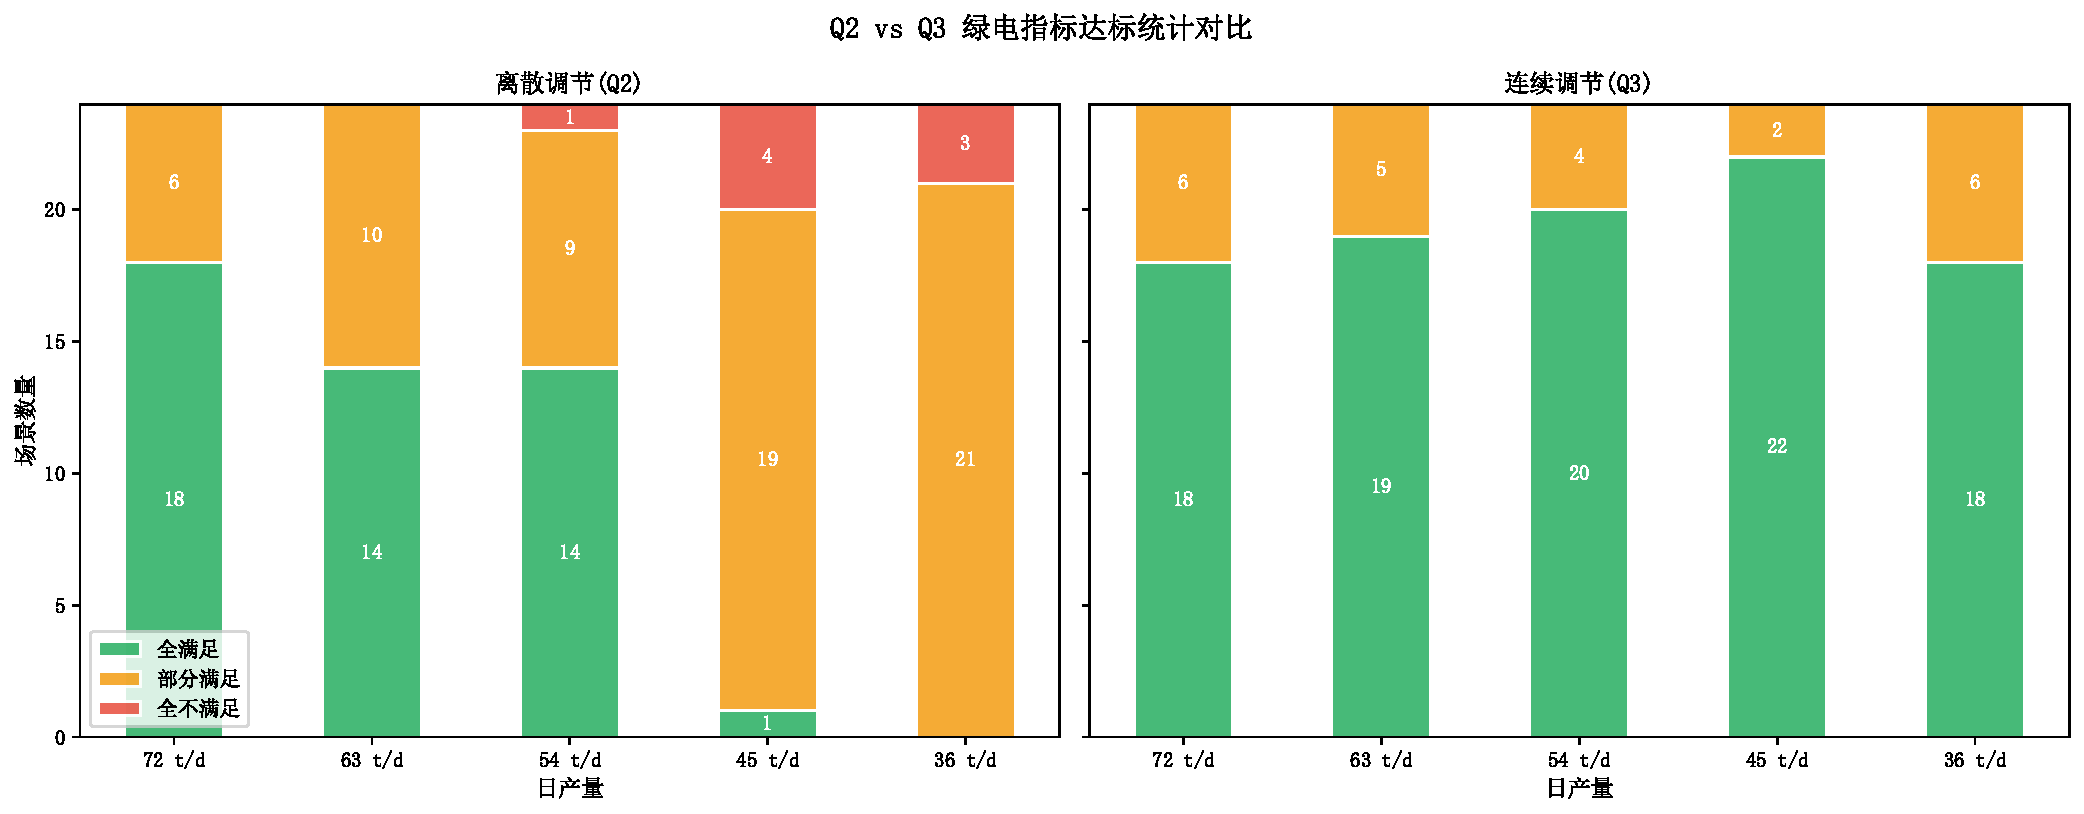
\includegraphics[width=\textwidth]{../figures/q3/fig12_q3_vs_q2_compliance.pdf}
\caption{Q2 vs Q3绿电指标达标统计对比}
\label{fig:q12_compliance}
\end{figure}

\cref{fig:q10_comparison}从成本角度对比了两种调节方式。连续调节在各产量下的吨氨成本略高于离散调节（约200-400元/吨），这是因为连续调节不再大量出售可再生余电，而是将其用于替代网购电力，虽然增加了自发自用电量、改善了绿电指标，但也减少了售电收益。以45 t/d为例，离散调节下售电收益较高使得成本低至3,945元/吨，但自用比例仅51.0%；连续调节下售电收益减少，成本升至4,005元/吨，但自用比例恢复到82.4%。

\cref{fig:q12_compliance}从达标角度展示了连续调节的压倒性优势。72 t/d时两种方式一致（均为18个全满足），但随着产量降低，离散调节的全满足数量急剧下降（45 t/d仅1个、36 t/d为0个），而连续调节的全满足数始终保持在18-22个的高水平。特别值得注意的是45 t/d这一产量——离散调节仅1个场景全满足，而连续调节高达22个。具体数量如\cref{tab:q3_compliance}所示。

\begin{table}[H]
\centering
\caption{Q2与Q3达标场景数对比}
\label{tab:q3_compliance}
\begin{tabular*}{\textwidth}{@{\extracolsep{\fill}}ccccccc}
\toprule[1.5pt]
产量 & \multicolumn{2}{c}{全满足} & \multicolumn{2}{c}{部分满足} & \multicolumn{2}{c}{全不满足} \\
(t/d) & Q2 & Q3 & Q2 & Q3 & Q2 & Q3 \\
\midrule[1pt]
72 & 18 & 18 & 6 & 6 & 0 & 0 \\
63 & 14 & 19 & 10 & 5 & 0 & 0 \\
54 & 14 & 20 & 9 & 4 & 1 & 0 \\
45 & 1 & 22 & 19 & 2 & 4 & 0 \\
36 & 0 & 18 & 21 & 6 & 3 & 0 \\
\bottomrule[1.5pt]
\end{tabular*}
\end{table}
